\chapter{Introduction}
\emph{The chapter starts with a background describing why road condition monitoring is important and who Trafikverket are, how road condition data is collected today and why the technology behind it needs improvement. Later on, machine learning basics are explained and how it can be used in this project. An objective for the project is defined followed by its delimitations. Lastly, a thesis structure is presented to simplify navigation through different parts of the project.}

\section{Background} \label{sec:background}
	Living in cold areas of the world usually means work for invididual people, municipalities and companies in trying to maintain a non-winter-like infrastructure. This of course, also involves winter road maintenance. Salting and plowing roads is an investment in not only saving lives, but also in lowering socio-economic costs; Arvidsson \cite{ARTICLE:1} presented two scenarios which explains this claim: The two scenarios take place on a road with 2 cm snow and a daily traffic flow of 2000 vehicles, one with a salted and ploughed road taking four hours to drive, and the other scenario on the same road without winter maintenance taking five hours to drive. Arvidson argues that the total socio-economic costs are 3.5\% higher in the non-maintained road, mainly due to increased travel time and thus higher accident costs. 


	\subsection{Road Weather Information Systems}
	While the socio-economic savings in performing winter road maintenance may be enough to justify why it's needed, it can still present a notable economic cost for the organization(s) involved. Trafikverket, the agency in charge of road state road maintenance in Sweden, reported that winter road maintenance were roughly 18\% of the total road maintenance costs in 2013 \cite{REPORT:1}. Local contracters are hired to carry out the plowing and salting of state roads, with requirements on both ends regarding when to plow, which roads to prioritize etc \cite{WEBSITE:2}. Trafikverket helps the contracters monitor road conditions with their so-called Road Weather Information System (RWIS) \cite{WEBSITE:2}. Trafikverket has around 800 RWIS (see \ref{img:rwis}) distributed across state roads in Sweden which are used by contracters to carry out winter road maintenance work \cite{WEBSITE:2}. 

\begin{figure}[H]
	\centering
	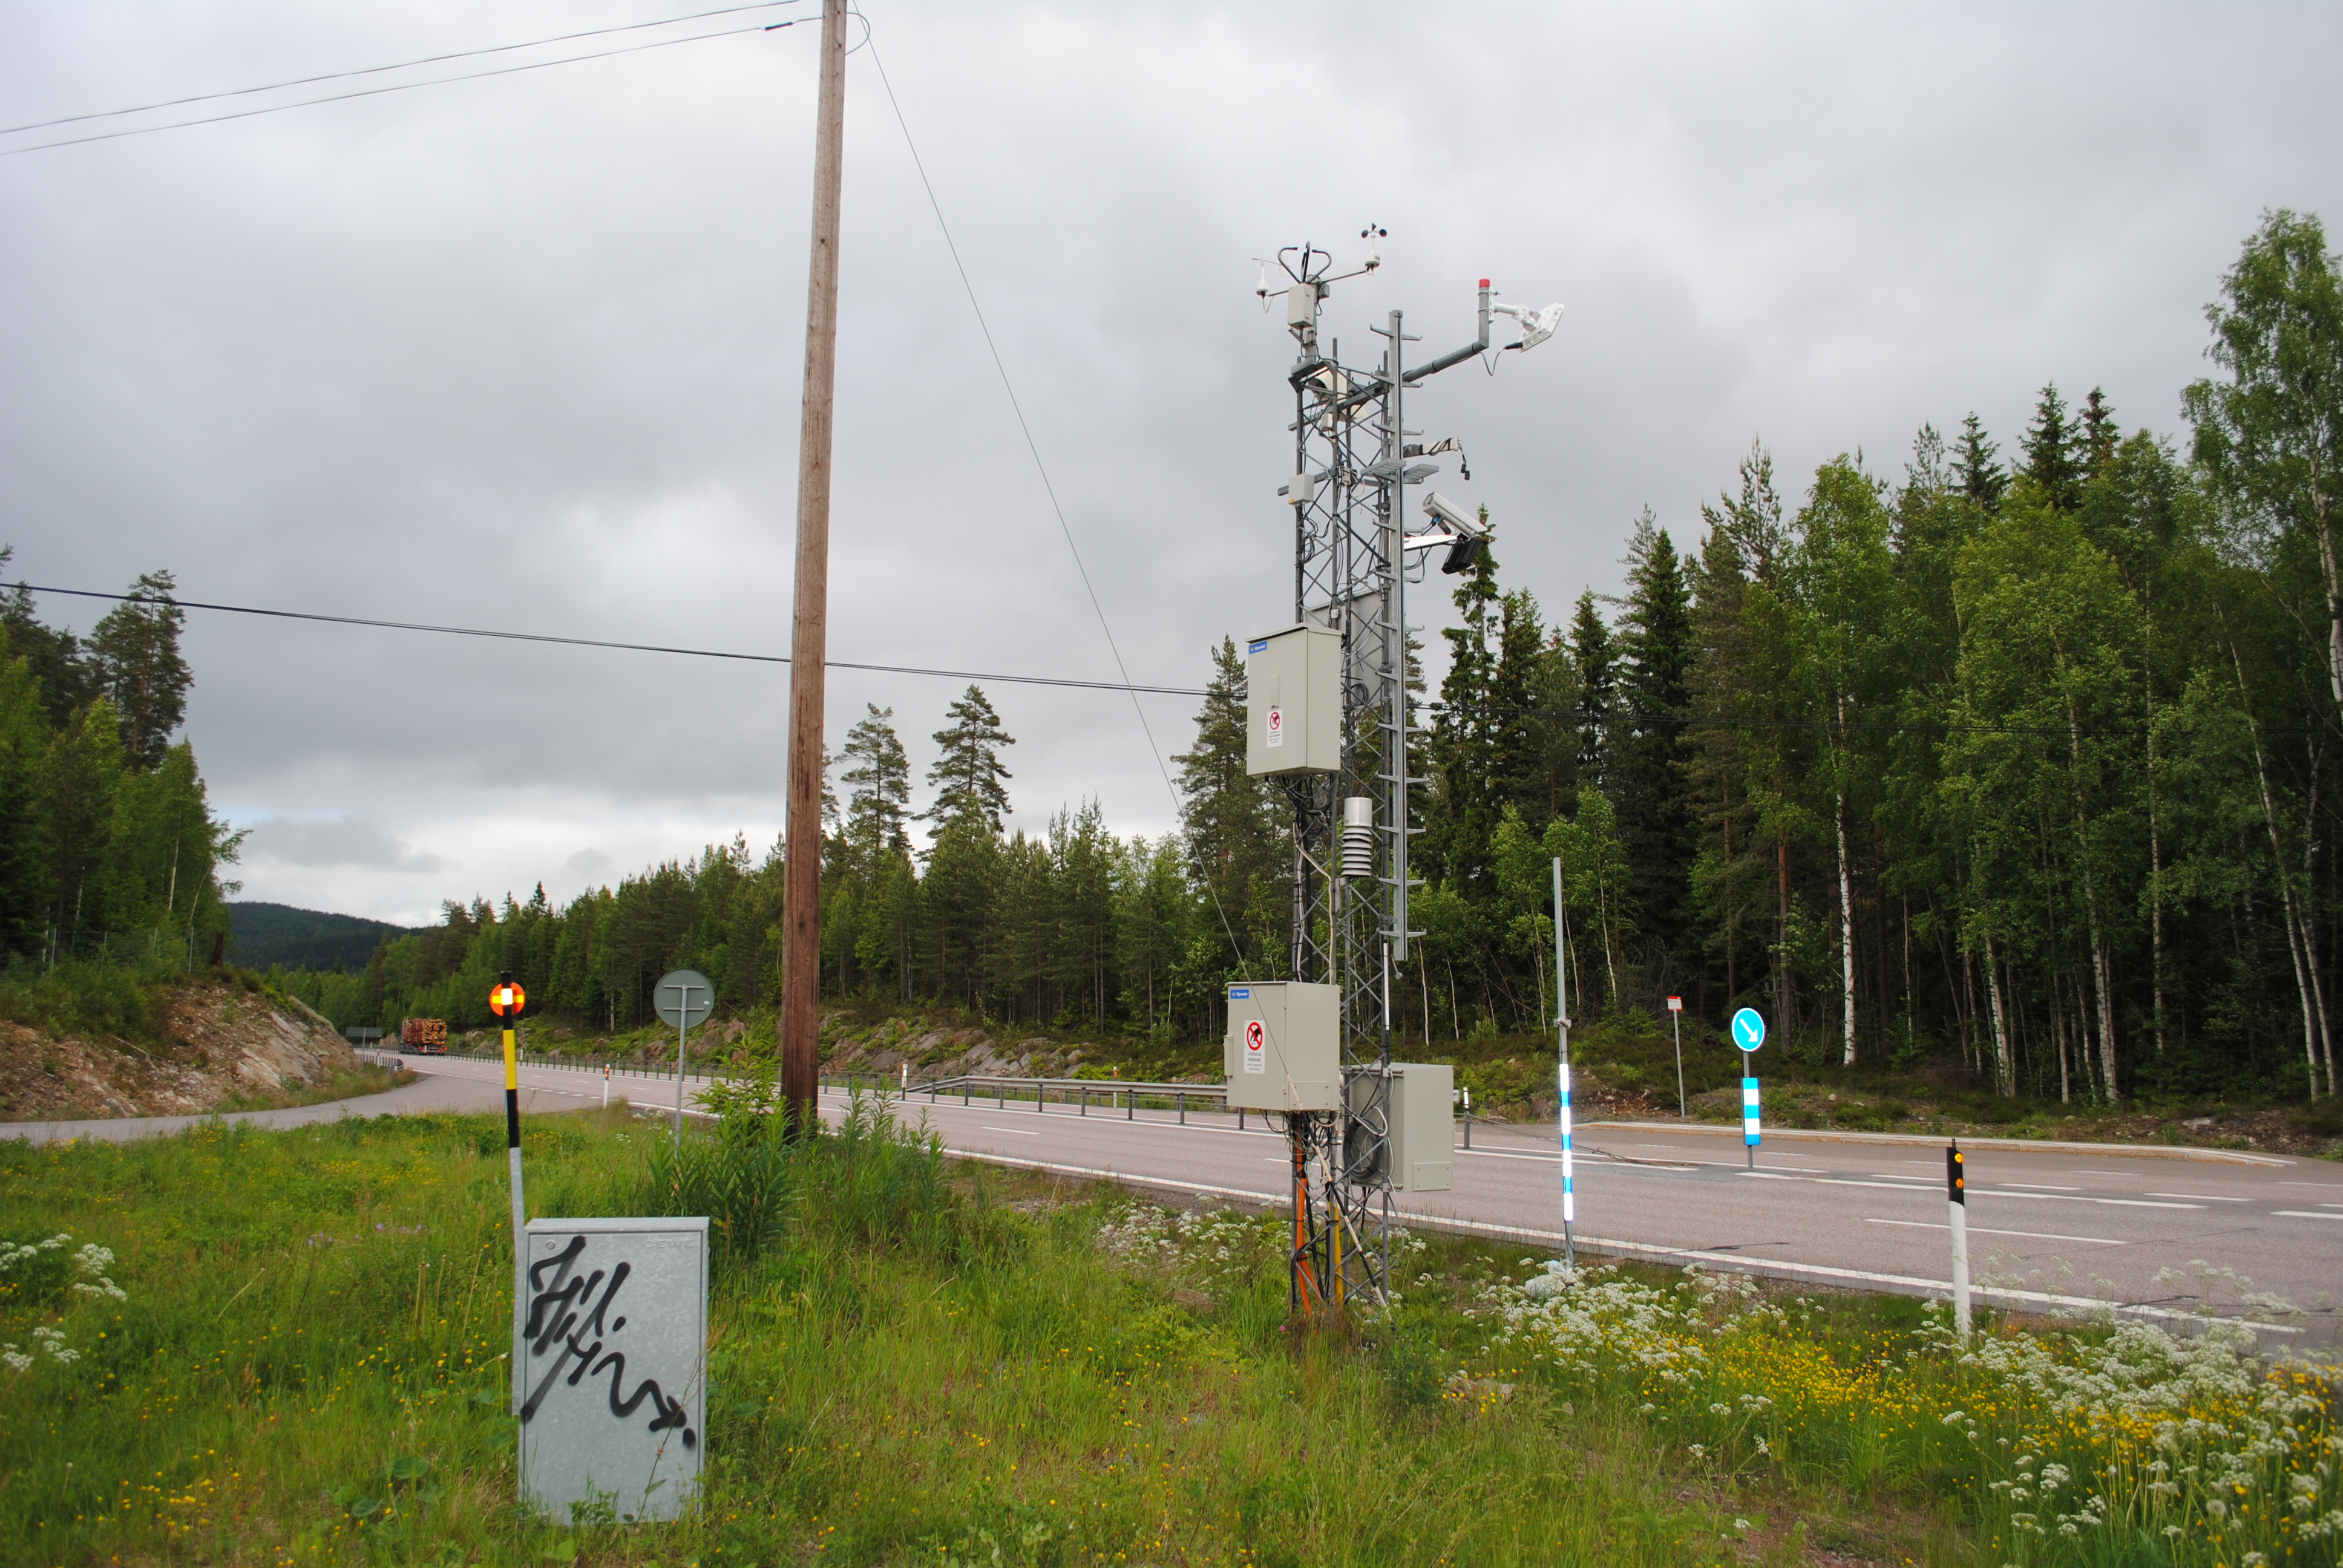
\includegraphics[width=0.8\textwidth]{media/Rwis_station_Myggsjon_01.JPG}
	\caption{RWIS Station at sensor site Myggsjön \cite{IMAGE:1}.}
	\label{img:rwis}
\end{figure}

\begin{table}[H]
	\caption{Measurements that are studied in this project from RWIS with corresponding instrument/sensor names\cite{MAIL:1, REPORT:3}. }
 	\resizebox{\textwidth}{!}{%
		\begin{tabular}[3]{l | l | l | l}
    			Instrument/sensor name & Feature & Value & Measured at how many RWIS  \\
    			\hline
			Optic Eye & precipitation type & discrete & all \\
			Optic Eye & precipitation amount & continous & all \\
			Track Ice Road Sensor & road surface temperature & continous & all \\
			DST111 & road surface temperature & continous & $\sim 7$ \\
			DSC111 & road surface condition & discrete &  $\sim 26$ \\
			DSC111 & road friction & continous & $\sim 26$ \\
			MS4 & measurement timestamp  & date (mmddhhmm) & all \\
			\label{table:rwis}
		\end{tabular}
		}
\end{table}

	Table \ref{table:rwis} shows some of the sensors the operational RWIS uses. The sensors are connected to a computer nearby computer called MS4, but Trafikverket aims to replace MS4 with a new generation of computers by 2021 \cite{REPORT:4}. The computer has limited capacity to handle current and future contracter needs, such as real-time image transfers, and electric components are hard to replace \cite{REPORT:4}. 

	In a personal interview with Johan Casselgren at Luleå University of Technology, he mentions that it is interesting to investigate if certain sensors, especially the Track Ice Road Sensor, can be replaced along with the new generation of computers. Johan Casselgren says that the Track Ice Road Sensors are dug into the road, which may require the road to be closed off temporarily during installation. Furthermore, if the sensor is removed, a hole is left in the road which can cause problems. In that way, the DST111 may prove useful since it measures road temperature remotely using infrared laser \cite{WEBSITE:19}. %but TIRS data still needed? why?
	%efter år 2022 bör inga givare finnas i vägbanan \
In addition to the sensors listed in \ref{table:rwis}, many of the stations are also equipped with a camera \cite{REPORT:2}. The operational RWIS also measure air humidity, air temperature, max-wind, wind-average and more, but neither these additional features nor the road photos taken by the camera are considered in this project since Johan Casselgren expressed an interest in investigating the relationship between the features in \ref{table:rwis}. Moreover, adding additional features may introduce the curse of dimensionality as brought up in \ref{sec:machinelearning}. 

The author, Johan Casselgren and Niklas Karvonen, who is also from Luleå University of Technology, concluded over personal communication that machine learning models can most likely be used to model the behavior of the Track Ice Road Sensor, and consequently, refrain from installing it in the future. The author and Johan Casselgren also sees potential in using machine learning models as a backup system when sensors malfunction, and therefore see benefits of modelling other sensors from \ref{table:rwis} as well. 

%lägg till ref till table som visar att dom failar ganska ofta

	\subsection{Machine learning} \label{sec:machinelearning}
	Machine learning as formally defined by Mitchell \cite{BOOK:2}: 
"A computer program is said to learn from experience $E$ with respect to some class of tasks $T$ and performance measure $P$ if its performance at tasks in $T$, as measured by $P$, improves with experience $E$". This means that machine learning algorithms are used to solve a set of problems, measure its performance in doing so and ultimately improve in some way from previous experiences. For example, imagine a program designed to determine if a human face is in a photo or not. Since photos are taken at different distances, angles and faces have different characteristics such as eye color, skin color, distance between eyes and nose shape, implementing this "manually" may prove cumbersome. Instead of programming an algorithm to recognize faces, it can be programmed  \emph{to learn to recognize faces}. If the algorithm is allowed to analyze a dataset with thousands of photos of human faces, it could learn to distinguish a human face by recognizing parts of the face such as eyes, nose, mouth and where those parts are most likely placed to oneanother.

	In essence, machine learning algorithms improve/learn in some way from analyzing a dataset. How they learn can be used to broadly categorize machine learning algorithms as either having supervised or unsupervised learning \cite{BOOK:1}. Supervised learning algorithms processes a labeled dataset while unsupervised learning attempts to make sense of unlabeled data. As can be seen in \ref{sec:provided_data}, the data provided by Trafikverket to perform this project is labeled data in the form of column headers in Microsoft Excel workbooks.  If, for some reason, the column headers were to be removed, it would qualify as an unlabeled dataset. Given that a labeled dataset is provided in this project, it makes sense to consider supervised learning algorithms.

	Dimensionality in machine learning refers to how many features are used as input to the algorithm. A one dimensional dataset could for example contain 171425 observations with one feature: precipitation type. A tempting brute-force approach may be to include every possible feature available, not only those brought up in \ref{table:rwis}, but also road photos, wind-speed etc. This however, may lead to something called the curse of dimensionality, which basically means that more dimensions in the dataset introduces complexity and possibly an increased amount of erros in the model \cite{BOOK:6}. During a personal meeting, Johan Casselgren also recommended to focus on using the features listed in \ref{table:rwis}. However, over an email conversation with Jonas Hallenberg who works at Trafikverket, difficulties were expressed in trying to model the DSC111 sensor. He says the problem is that Trafikverket uses salt on all the of the roads where the DSC111 sensor is, save one, and salt affects the road surface status. So for example when the surface temperature and dew point temperature suggests the road surface condition is icy, which could be measured by DSC111, it may in fact be wet in reality. Johan casselgren suggests that data from DSC111 can be used to model the other sensors. Data from the Track Ice Road Sensor road temperature is not to be used as input when modelling remaining sensors since, as previously covered, Trafikverket plans rid of this sensor in the future. 
	
	The forementioned definition of machine learning by \cite{BOOK:2} mentions a performance measure $P$. This measure can be used to evaluate supervised learning algorithm's abilities to model a feature in \ref{table:rwis}, see \ref{sec:supervisedlearning} for more information on performance measures. A specific feature that is to be modelled is referred to as target feature, and the features a supervised learning algorithm uses to do so is referred to as input features. In a basic sense, a supervised learning algorithm studies the observations of the target feature as a mathematical graph and attempts to build a model that best fits the observations in the graph. But the algorithm is not necessarily perfect by having a high performance score. If the model is built in such a way that it fits the provided data perfectly, which may have outliers etc, it may have difficulties in predicting new data. This condition is known as overfitting, the opposite is called underfitting, both of which are covered in detail in \ref{sec:generalization}. So not only is an algorithm with high performance desirable, also one whose model generalizes well so that both underfitting and overfitting is avoided.

\section{Objective}
	The objective is to find supervised learning algorithms that best models the observations made by the following sensors: Optic Eye, Track Ice Road Sensor, DST111 and DSC111 in terms of performance and generalization. The objective is broken down into four tasks:
	
	\begin{enumerate}
		\item Find the algorithm among supervised learning algorithms, that can be used to classify \textbf{precipitation type}, whose performance and generalization score is highest. The data may contain the following input features: 
			\begin{itemize}
				\item measurement timestamp
				\item DST111 road surface temperature
				\item road friction
				\item road surface condition
			\end{itemize}
		\item Find the algorithm among supervised learning algorithms, that can be used to predict \textbf{precipitation amount}, whose performance and generalization score is highest. The data may contain the following input features: 
			\begin{itemize}
				\item measurement timestamp
				\item DST111 road surface temperature
				\item road friction
				\item road surface condition
			\end{itemize}
		\item Find the algorithm among supervised learning algorithms, that can be used to predict \textbf{Track Ice Road Sensor road surface temperature}, whose performance and generalization score is highest. The data may contain the following input features: 
			\begin{itemize}
				\item measurement timestamp
				\item precipitation type
				\item precipitation amount
				\item DST111 road surface temperature
				\item road friction
				\item road surface condition
			\end{itemize}
		\item Find the algorithm among supervised learning algorithms, that can be used to predict \textbf{DST111 road surface temperature}, whose performance and generalization score is highest. The data may contain the following input features: 
			\begin{itemize}
				\item measurement timestamp
				\item precipitation type
				\item precipitation amount
				\item road friction
				\item road surface condition
			\end{itemize}
	\end{enumerate}

\section{Delimitations} \label{sec:delimitations}
	There are many supervised learning algorithms, all of which are not evaluated in detail in this project. An algorithm is qualified for evaluation in this project if the following is true:
	\begin{enumerate}
		\item The algorithm is a supervised learning algorithm that solves regression and/or multiclass classification problems (see \ref{sec:classification} and \ref{sec:regression})
		\item The algorithm is available in Scikit-learn \cite{WEBSITE:15}
		\item The algorithm belongs to one of the following algorithm families (see \ref{sec:supervised_algorithms}):
			\begin{itemize}
				\item Decision tree based learning %cart
				\item Instance based learning %knn
				%\item Kernel methods based learning %svm
				\item Bayesian learning %GaussianNB
				\item Regression based learning %linear regression, logistic regression, lasso?
				\item Deep learning %backpropagation
				\item Ensemble learning %random forest
			\end{itemize}
	\end{enumerate}

	The performance of supervised algorithms can generally be improved by optimizing its hyperparameters (see \ref{sec:hyperparameters}). However, there can be many ways that a single algorithm can be configured. Since this project deals with comparing performances of several algorithms, exploring all combination of hyperparameters would take a significant amount of time both in setting up experiments, and in actual running-time. When it comes to optimizing hyperparameters, it was decided to focus on the choice of $k$ in kNN, the number of hidden nodes in Backpropagation, and magnitude of regularization $\lambda$ in Lasso (see \ref{sec:supervised_algorithms} and \ref{sec:regularization}).
 
	Some of the sensors, such as the DSC111 (see \ref{img:histogram_surfstatus}), are malfunctioning frequently. To avoid any complex relationships between functioning and malfunctioning sensors, it is decided to model non-error behavior by using non-error input features only. 

	In addition to the time feature, an extra feature was present in the provided dataset which displayed what year each observation was taken. The author assumes that global warming does not present a significant change in weather conditions, road surface temperature etc. such that 2015 and 2016 are relatively similar in that sense. Also since the measurements are from 2015-2016, it is assumed that any model built using year as input feature could potentially do well when dealing with new observations whose year is 2015 or 2016 but that it generalizes poorly when dealing with observations from 2018 etc. By these assumptions, it was decided to not consider year as an input feature. 

	Support vector machine (SVM) algorithms could have been evaluated in this project, but was ruled out since they appear to have high computational running-time. It was revealed by the author, through a cross-validation classification spot-checking test (see \ref{sec:exp_setups}) on the iris dataset in Scikit-learn, that SVM have significantly longer running-time than the other algorithms in \ref{table:evaluated_algorithms}.


\section{Provided data} \label{sec:provided_data}
	A dataset containing 171425 measurements (observations) was provided by Trafikverket to carry out this project. The observations are from 2015-2016 from six RWIS along state road E6 in Sweden, where every station measures the features seen in \ref{table:rwis} roughly every 30 minutes. Six Microsoft Excel workbooks represent data from each of the six stations, in which the column headers are the features seen in \ref{table:rwis}. The year each observation was taken is also represented in a column in the workbooks.

	A readme.txt file was also provided. It explains in words how to interpret the observations. As can be seen in \ref{table:rwis}, precipitation type and road surface condition have discrete values that are explained in the readme file.
		
\begin{table}[H]
	\caption{Values that Optic Eye precipitation type and DSC111 road surface condition can assume and what they mean.}
 	\resizebox{\textwidth}{!}{%
		\begin{tabular}[3]{l | l | l}
    			Value & Precipitation type & Road surface condition \\
    			\hline
			-9 & missing sensor/error & - \\
			0 & - & error\\
			1 & no precipitation & dry \\
			2 & rain with $>= 0 \celsius$ air temperature & moist \\
			3 & rain with $< 0 \celsius$ air temperature & wet \\
			4 & snow & - \\
			5 & - & frost \\
			6 & rain and snow mixed  & snow \\
			7 & - & ice \\
			9 & unknown type  & slush \\
			\label{table:discretevalues}
		\end{tabular}
		}
\end{table}

\section{Thesis structure}
% explain what the thesis looks like
